\documentclass{standalone}
\usepackage{tikz}
\usepackage{ctex,siunitx}
\usepackage{tkz-euclide}
\usepackage{amsmath}
\usetikzlibrary{patterns, calc}
\usetikzlibrary {decorations.pathmorphing, decorations.pathreplacing, decorations.shapes,}
\begin{document}
\small
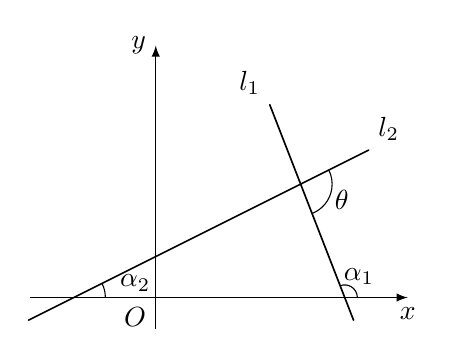
\begin{tikzpicture}[>=latex,scale=0.8]
  \begin{scope}
    \draw[thin,->](-2,0)--(4,0)node[below]{$x$};
    \draw[thin,->](0,-0.5)--(0,4.0)node[left]{$y$};
    \tkzDefPoints{-1.3/0/A,3.0/0/B,2.3/1.8/C,0/0/O,5/0/P}
    \tkzDefPointOnLine[pos=1.5](A,C)\tkzGetPoint{D}
    \tkzDefPointOnLine[pos=1.5](B,C)\tkzGetPoint{E}
    \tkzDrawLine[semithick,add = 0.2 and 0.7](B,C)
    \tkzLabelLine[pos=1.7,above left](B,C){$l_1$}
    \tkzDrawLine[semithick,add = 0.2 and 0.3](A,C)
    \tkzLabelLine[pos=1.3,above right](A,C){$l_2$}
    \tkzMarkAngle[size=0.5](B,C,D)
    \tkzLabelAngle[pos=0.7](B,C,D){$\theta$}
    \tkzMarkAngle[size=0.5](P,A,C)
    \tkzLabelAngle[pos=1.0](P,A,C){$\alpha_2$}
    \tkzMarkAngle[size=0.2](P,B,C)
    \tkzLabelAngle[pos=0.4](P,B,C){$\alpha_1$}
    \tkzLabelPoints[below left](O)
  \end{scope}
\end{tikzpicture}
\end{document}